\documentclass[a4paper, 11pt]{article}
\usepackage[utf8]{inputenc}
\usepackage[T1]{fontenc}

\usepackage{amsmath} \usepackage{amsthm} \usepackage{bm} \usepackage{graphicx}
\usepackage[usenames, dvipsnames]{xcolor} \usepackage{enumitem}
\usepackage{caption} \usepackage{subcaption} \usepackage{float}

\usepackage{mathpazo} \usepackage{geometry} \usepackage{setspace}

\usepackage[colorlinks=true]{hyperref} \newcommand\myshade{100}
\colorlet{myblue}{NavyBlue} \colorlet{mybrown}{OrangeRed}
\colorlet{mygreen}{ForestGreen}

\hypersetup{ linkcolor = mybrown!\myshade!black, citecolor =
  myblue!\myshade!black, urlcolor = mygreen!\myshade!black, colorlinks = true, }

\usepackage[round]{natbib} \bibliographystyle{apalike}

\newtheorem{theorem}{Theorem} \newtheorem{principle}{Principle}
\newtheorem{proposition}{Proposition} \theoremstyle{remark}
\newtheorem{example}{Example}

\usepackage{amssymb}
\begin{document}

\title{Model and estimators for partial least squares.\\
  Running title: Model and estimators for PLS.}

\author{Helland, I.S., University of Oslo,  S\ae b\o , S., Alm\o y, T.  and Rimal, R.,\\
  Norwegian University of Life Sciences}

\maketitle

\begin{abstract}

\end{abstract}

\setcounter{tocdepth}{1}
\tableofcontents

\onehalfspacing
 
\section{Introduction}

Supervised learning from multivariate data is a central problem area in applied
statistics. Specifically, let our task be to predict a sinwidtgle variable $y$ from
a $p$-dimensional variable $\bm{x}$, having data on $n$ units. A large number of
learning methods are discussed in \citet{hastie2009elements}, mainly under the
ordinary multiple regression model. It is part of the philosophy of the present
paper that for near collinear data, a \emph{reduction} of the regression model
is called for.

Here we will take as our point of departure a well defined reduction of the
random $\bm{x}$ regression model, the envelope model of
\citet{cook2013envelopes} Cook et al (2013). In op. cit. it has been shown in
detail that the envelope model in the case of reduction in the $\bm{x}$-variable
is equivalent to the partial least square population model of
\citet{helland1990partial} Helland (1990), and that a corresponding result is
also valid in the case of a multivariate $\bm{y}$.

Partial least squares (PLS) regression has had a vigorous devolopment in the
chemometric literature since it was proposed by Herman and Svante Wold and by
Harald Martens \citep{wold1984collinearity, martens1992multivariate} (Wold et
al, 1984; Martens \& N\ae s, 1992). The method has been extended in several
directions and its applications have been expanded to an increasing number of
fields, for instance genomic data \citep{boulesteix2007partial}. Both these
issues have been discussed in detail in a recent paper by
\citet{mehmood2016diversity}, where a wealth of further references may be found.

In the beginning the PLS method was to some extent neglected or turned down by
statisticians (an exception among others was \citealp*{frank1993statistical}),
but it is now included as a tool among other biased regression methods by
applied statisticians. For a general discussion paper with contributions both
from mathematical statisticians and chemometricians, see
\citet{sundberg1999multivariate}.

Indeed there was a difference in culture between chemometricians and
statisticians then, and this difference still exists to a large extent. A recent
statement by \citet{munck2010physiochemical} illustrates this: 'If chemometrics
in its historical development had been limited to follow current scientific (and
statistical) theories there would have been minimal progress in its wide
applications today.'

This difference in culture may be related to the concepts of creativity and
rigor, qualities which to some extent may be called complementary. One could say
that one culture puts more emphasis on creativity, the other on rigor. Of
course, this is a huge simplification. First, there is a lot of creativity among
statisticians, also mathematical statisticians. Secondly, one should emphasize
that precise thinking also should influence practice. A case of point is the
following: \citet{chung2010sparse} recently proved that the PLS regression
vector is inconsistent when there is noise in the $x$-variables when
$p/n\rightarrow k>0$. This result is probably not too well known among
chemometricians; some may have a tendency to put too much confidence in PLS
regression when $p\sim n$ or $p>n$, also in cases where there may be noise in
the $x$-variables.

However, it is true that chemometricians have had a leading edge in the
development of PLS and of certain multivariate methods, in particular with
respect to visualization etc., and they still may be ahead of us in this sense,
even though there is a growing literature in statistical journals on the
envelope model and on estimation in this model; see below.

Accepting this, an important general question is what mathematical statisticians
can contribute with in this development. A vital aspect in the history of
statistics is the interplay between model and estimators. Once a model is
formulated, one can in principle think of several estimators in this model. Thus
in the PLS/envelope model one can certainly discuss other estimators than the
usual PLS regression estimator, which can be seen as originating by replacing
population (co-)variances in the model by sample (co-)variances. Two examples
are the maximum likelihood estimator of \citet{cook2013envelopes}, see also
\citet{cook2015envlp}, \citet{cook2016note} and \citet{cook2016algorithms}; and
the Bayesian estimator of \citet{helland2012near}. By simulation, both these
estimators have performed well compared to PLS regression, but they have their
disadvantages. The maximum likelihood estimator can not be used in the important
case when the data matrix has rank less than $p$, and the Bayesian estimator
requires heavy computations, in particular when $p$ is large.

To compare estimators we make vital use of the recently developed simulation
package simrel; see \citet{saebo2015simrel}. A main purpose of the present paper
is to illustrate the interplay between mathematical arguments on the one hand
and systematic simulations on the other hand in an area where it is difficult to
obtain results by purely analytical means.

It is important to emphasize that this paper is based upon reduction of the
\emph{random} $\bm{x}$ regression model. When considering latent variables from
PLS, and when considering near collinearity in the observed $\bm{x}$-variables,
it is natural to treat these $\bm{x}$-variables as random. It is our philosophy
that this is also the best way to look upon model reduction. On the other hand,
in the context of prediction, one could argue that one should condition upon the
$\bm{x}$-variables and consider them as fixed. A prominent paper on PLS
regression, taking fixed $\bm{x}$-variables in the basic model, is
\citet{kramer2012degrees}, where further references can be found.

In recent years there has been a rapidly growing literature on the envelope
model. In addition to the maximum likelihood estimation paper mentioned above,
the most important papers seem to be \citet{cook2015simultaneous}, where
simultaneous reduction in the $\bm{x}$-space and $\bm{y}$-space is proposed, and
\citet{cook2015foundations}, where extensions to other regression methods than
linear regression are discussed. More references can be found in these papers.

The plan or this paper is as follows:

\section{The model}

\subsection{Several formulations}

Take as a point of departure the linear model
\begin{equation}
  \label{model}
  y=\mu_{y}+\bm{\beta}'(\bm{x}-\bm{\mu}_{x})+\epsilon,
\end{equation}
where $\bm{\beta}$ and $\bm{x}$ are $p$-dimensional, and where the random predictor $\bm{x}$ has mean $\bm{\mu}_{x}$ and covariance matrix $\bm{\Sigma}_{xx}$, for simplicity assumed nonsingular here. (This can be relaxed to assuming $\bm{\beta}\in\mathrm{span}(\bm{\Sigma}_{xx})$ in the case where this matrix is singular; see \citet{cook2013envelopes}, and also C below.) Independently, $\epsilon$ is distributed with mean $0$ and variance $\sigma^2$. When doing prediction from this model for near collinear data, a model reduction may be called for. Throughout this paper, a definite $m$-dimensional model reduction, which may be formalized in several equivalent ways, will be used. When this model holds, we say that we have an envelope model of dimension $m$, or that there are $m$ relevant components for prediction in the model.
\smallskip

\begin{enumerate}[label=\Alph*.]

\item Given a subspace $\cal{T}$ of $R^p$, let $\bm{P}_{\cal{T}}$ be the projection upon $\cal{T}$, and let $\bm{Q}_{\cal{T}}$ be the projection orthogonal to $\cal{T}$. Let now $\cal{T}$ be the smallest space such that (i) $\bm{Q}_{\cal{T}}\bm{x}$ is uncorrelated with $\bm{P}_{\cal{T}}\bm{x}$; (ii) $y$ is uncorrelated with $\bm{Q}_{\cal{T}}\bm{x}$ given $\bm{P}_{\cal{T}}\bm{x}$. In this case we may say that $\bm{Q}_{\cal{T}}\bm{x}$ contains no information about $y$, neither directly nor through $\bm{P}_{\cal{T}}\bm{x}$. Here $\cal{T}$ must be seen as a subspace of the $x$-space. Let $\cal{S}$ be the corresponding dual subspace of the parameter-space: Define $\cal{S}^\perp$ as the set of $\bm{\gamma}$ such that $\bm{\gamma}'\bm{x}=0$ for all $\bm{x}\in\cal{T}$, and let $\cal{S}$ be the space perpendicular to $\cal{S}^\perp$. 
  \smallskip

\item  Here is an algebraic characterization which turns out to be equivalent. For a matrix $\bm{M}$ define $\bm{M}\cal{S}$ as the space of vectors $\bm{Mz}$ as $\bm{z}$ runs through $\cal{S}$, and let $\cal{S}^\perp$ be 
  the space perpendicular to $\cal{S}$. Let now $\cal{S}$ be the smallest space in $R^p$ such that (i) both $\bm{\Sigma}_{xx}\cal{S}\subseteq\cal{S}$ and 
  $\bm{\Sigma}_{xx}\cal{S}^\perp\subseteq\cal{S}^\perp$; (ii) $\mathrm{span}(\bm{\beta})\subseteq\cal{S}$. In this case we say that $\cal{S}$ 
  is the envelope of $\mathrm{span}(\bm{\beta})$. It can be shown (Cook et al, 2010) that the envelope always exists as the smallest space with the stated properties.
  \smallskip

\item The regression vector $\bm{\beta}$ can always be expanded in terms of the eigenvectors $\bm{d}_{i}$ of $\bm{\Sigma}_{xx}$: 
  $\bm{\beta}=\sum_{i=1}^p \gamma_{i}\bm{d}_{i}$. Assume that this sum can be reduced to exactly $m$ non-zero terms:
  $\bm{\beta}=\sum_{i=1}^m \gamma_{i}\bm{d}_{i}$, where the $\bm{d}_i$ correspond to different eigenvalues of $\bm{\Sigma}_{xx}$. We then say that there are $m$ relevant components for prediction in the model. This reduction can be imagined to take place by two mechanisms: 1) Some of the $\gamma_i$'s are really zero. 2) There are coinciding eigenvalues in $\bm{\Sigma}_{xx}$. Then one can rotate such that it is enough with one eigenvector for each eigenspace in the sum. In this approach it is important that we only know that there are $m$ non-zero terms in the sum, not which  terms that are non-zero. For a closer discussion of this, see N\ae s \& Helland (1993) and Helland \& Alm\o y (1994).
  \smallskip

\item Consider the  population version of the well known PLS algorithm: Take 
  $\bm{e}_{0}=\bm{x}-\bm{\mu}_{x}$, $f_{0}=y-\mu_{y}$, and for $a=1,2,...,m$ compute successively: 
  \begin{equation} \label{wt}\bm{w}_{a}=\mathrm{cov}(\bm{e}_{a-1}, f_{a-1}),\ \ \  
    t_{a}=\bm{w}_{a}'\bm{e}_{a-1},\end{equation}
  \begin{equation}\label{pq}\bm{p}_{a}=\mathrm{cov}(\bm{e}_{a-1}, t_{a})/\mathrm{var}(t_{a}),\ \ 
    q_{a}=\mathrm{cov}(f_{a-1},t_{a})/\mathrm{var}(t_{a}),\end{equation}
  \[\bm{e}_{a}=\bm{e}_{a-1}-\bm{p}_{a}t_{a},\ \ \ 
    f_{a}=f_{a-1}-q_{a}t_{a}.\]
  It can be proved (Helland, 1990), and is important in this connection that under the reduced model C, this algorithm stops automatically after $m$ steps when 
  $m<p$: It stops because $\bm{w}_{m+1}=\mathrm{cov}(\bm{e}_{m},f_{m})=0$. After those $m$ steps we get the representations

  \begin{equation}
    \label{latent}
    \bm{x}=\bm{\mu}_{x}+\bm{p}_{1}t_{1}+...+\bm{p}_{m}t_{m}+\bm{e}_{m},\ \ y=\mu_{y}+q_{1}t_{1}+...+q_{m}t_{m}+ f_{m}
  \end{equation}

  with the corresponding PLS population prediction

  \[y_{m,PLS}=\mu_{y}+q_{1}t_{1}+...+q_{m}t_{m}=\mu_{y}+\bm{\beta}_{m,PLS}'(\bm{x}-\bm{\mu}_{x}).\]

\end{enumerate}

\smallskip

\begin{theorem} {\rm\citep{cook2013envelopes,helland1990partial}}
  \begin{enumerate}[label=(\alph*)]
  \item The two conditions A and B on the space $\cal{S}$ are equivalent.
  \item The models formulated by C and D are equivalent.
  \item When there are $m$ relevant components for prediction, the envelope space $\cal{S}$ has dimension $m$, and $\cal{S}$ can be taken as $\mathrm{span}\left(\bm{w}_{1}, \ldots, \bm{w}_{m}\right) = \mathrm{span}\left(\bm{d}_{1}, \ldots, \bm{d}_{m}\right)$.
  \item When the envelope space has dimension $m$, there are $m$ relevant components for prediction.
  \item In this case we have $\bm{\beta}_{m,PLS}=\bm{\beta}$.
  \end{enumerate}
\end{theorem}

\bigskip

In this sense all the model formulations A-D are equivalent; they describe the same reduced model. In \citet{cook2013envelopes}, a fifth equivalent formulation in terms 
of a Krylov sequence is also given. Being a reduced model that can be motivated in so many different ways, it is definitively of interest to find a good estimator of the regression vector $\bm{\beta}$ under this model.

\bigskip

\subsection{Could the PLS/envelope model have been developed earlier by statistical arguments?}

The PLS population model of \citet{helland1990partial} was motivated as a statistical interpretation of the chemometricians' PLS algoritm. The purpose of this subsection is to show that the same model could have been deduced by using symmetry consideration. Since model reduction from symmetry is a new way of thinking for many statisticians, we include several simple examples before returning to PLS.

In general a given statistical problem involving a parameter $\theta$ may often have some 
symmetry property associated with it, and this is formalized by introducing a group $G$ of transformations acting upon the parameter space $\Theta$. 

When $\theta$ is transformed by the group $G$ and the observations are transformed accordingly \citep[see][]{helland2004statistical}, one should get equivalent results from the statistical analysis. As a trivial example: One should get equivalent results from a statistical analysis whether the parameters and the observations are measured in meters or in centimeters. Examples of groups acting upon a parameter space, are location: $\xi\rightarrow \xi+a$ for $a$ real; scale group: $(\xi ,\sigma)\rightarrow (b\xi , b\sigma)$ for $b>0$; location and scale: $(\xi,\sigma)\rightarrow(a+b\xi, b\sigma)$, where $\xi$ is an expectation and $\sigma$ is a standard deviation; rotation in a multidimensional parameter space; a general linear group acting upon a multidimensional parameter space etc.. Invariance under a group may help improving the estimation or the inference in general.


We will not be very precise on the choice of $G$, but just say vaguely that we choose $G$, if possible, in agreement with some symmetry aspect of the whole situation.

Now fix a point $\theta_0$ in the parameter space $\Theta$. An \emph{orbit} in this space under $G$ is the set of points of the form $g\theta_0 $ as $g$ varies over the group $G$. The different orbits are disjoint, and $\theta_0$ 
can be replaced by any parameter on the orbit. Any set in $\Theta$ which is an orbit of $G$ or can be written as a union of orbits, is an invariant set under $G$ in $\Theta$, and conversely, all invariant sets can be written in 
this way. If there is only one orbit in $\Theta$, the group is said to be acting transitively upon $\Theta$.

A statistical model should be as simple as possible, but not simpler. In some cases we may want to do a simplification, a model reduction. This may take the form of a reduction of the parameter space $\Theta$. Parts of this space which 
are essential for the statistical analysis, must always be retained, but irrelevant dimensions should be left out. We will now formulate a general criterion which will be used throughout this subsection:
\bigskip

\begin{principle}
  \label{principle1}
  If there is a group $G$ acting upon the parameter space $\Theta$, any model reduction should be to an orbit or to a set of orbits of $G$.
\end{principle}

This will ensure that $G$ also can be seen as a group acting upon the new parameter space. In particular, if the group actions form a transitive group $G$, no model reduction is possible. A far more general theory on what should constitute a valid statistical model, is given by McCullagh (2002).
\bigskip

\begin{example}
  Assume that a single set of observations is modeled by some large parametric model, only assuming that parametric class contains the normal model. Let the location and scale group be acting upon the parameter space $\Theta$. Then one orbit is given by the normal distribution. This is not an uncommon model reduction.
\end{example}

\smallskip

\begin{example}
  Look at two independent sets of observations: $(x_1 ,...,x_m )$ independent and identically $N(\xi_1,\sigma_1^2)$ and $(y_1 ,...,y_n )$ independent and identically $N(\xi_2 , \sigma_2 ^2)$. Let $G$ be the translation and scale group given by $\xi_1 \rightarrow a_1 +b\xi_1 ,\ \sigma_1 \rightarrow b\sigma_1 , \ \xi_2 \rightarrow a_2 +b\xi_2 ,\ \sigma_2 \rightarrow b\sigma_2 $. 

  Note that a common scale transformation by $b$ is assumed. Then the orbits of the group in the parameter space are given by $\sigma_1 /\sigma_2 =\mathrm{constant}$. A common model reduction is given by $\sigma_1 =\sigma_2 $. This simplifies the comparison of $\xi_1 $ and $\xi_2 $, which is often the goal of the investigation.
\end{example}

\smallskip

\begin{example}
  Linear statistical models have a large range of applications. In general these models have the form where the observations $y_l$ are independent $N(\xi_l ,\sigma^2 )$, where the expectations $\xi_l$ are linear combination of a set of parameters. One particular such model is the two-way analysis of variance model, where the observations $y_{ijh}$ have expectations $\xi_{ij}=\mu +\alpha_i +\beta_j +\gamma_{ij}$. To get a unique representation of this kind, one usually imposes the restrictions $\sum_i \alpha_i =0$, $\sum_j \beta_j =0$, $\sum_i \gamma_{ij} =0$ for each $j$ and $\sum_j \gamma_{ij} =0$ for each $i$. Let the group $G$ be given by translations $\xi_{ij}\rightarrow\xi_{ij}+a_i+b_j$. Then a common model reduction is given by the invariant set where the expectation is $\mu +\alpha_i +\beta_j $. This is the model without interaction, and is a valid simplification in some cases. Note that in this setting, certain other formal model reductions, say letting the expectation be $\mu+\alpha_i +\gamma_{ij}$ are meaningless given this symmetry group.
\end{example}

\smallskip

\begin{example}
  Another example of a linear model is the polynomial regression model $y_i =\beta_0 + \beta_1 x_i +...+\beta_p x_{i}^p +\epsilon_i$, where the $\epsilon_i$'s are independent $N(0,\sigma ^2)$ for $i=1,...,n$. Let $G$ be the group defined by translations in the $x$-space: $x\rightarrow x+a$, which generates a transformation group on the parameters $(\beta_0 ,...,\beta_p )$. Then the submodels $y_i =\beta_0 + \beta_1 x_i +...+\beta_q x_{i}^q +\epsilon_i$ $q<p$ correspond to invariant sets in the parameter space, while many other polynomial submodels are not invariant under the group $G$. 
\end{example}

\smallskip

\begin{example}
  A further example of a linear model is the multiple regression model $y_i = \beta_0 +\beta_1 x_{i1}+...+\beta_p x_{ip} +\epsilon_i $ for $i=1,..,n$ with fixed $x_{ij}$, which again has many different applications. Consider first the case where the $x_{ij}$ are measured in different units for different $j$. Then there is a natural transformation group given by separate scale changes $x_{ij}\rightarrow k_j x_{ij}$ $(i=1,...,n; j=1,...,p)$. This induces a group on the regression parameters by $\beta_j \rightarrow \beta_j /k_j $ $(j=1,...,p)$. The invariant sets in the parameter space are found by putting some of the $\beta_j$'s equal to $0$. These reduced models are well-known from many applications of regression analysis. Note that many other formal model reductions do not make sense, say $\beta_1=\beta_2$ if $x_{i1}$ and $x_{i2}$ are measured in different units.
\end{example}

\smallskip

\begin{example}
  Consider the same multiple regression model as in Example 5, but assume now that the explanatory variables $x_{ij}$ all are measured in the same units. A large class of transformations $\bm{x}_{i\cdot}\rightarrow \bm{Qx}_{i\cdot}$ may then be of interest. In particular, an interesting case is when $\bm{Q}$ varies over the orthogonal matrices.
\end{example}

\smallskip

As here, and as in any linear model, estimates of the regression parameters can in principle be found by the method of least squares, which is equivalent to 
the maximum likelihood method. However, this method breaks down when one has collinearity problems such that the matrix which we need to invert in order to implement the least squares solution, is singular, and the method is unstable when this matrix is near singular. A large number of alternative estimation methods are proposed in the statistical literature to tackle this problem, see for instance \citet{hastie2009elements}, but it seems very difficult to decide which of these methods one should use in practice.

Look now at a modification of this model where the explanatory variables are random variables. Then the model can be written on the form (\ref{model}).  The regression vector $\bm{\beta}$ can always be expanded in terms of an orthogonal set of eigenvectors $\bm{d}_i$ of $\bm{\Sigma}_{xx}$:

\begin{equation}
  \bm{\beta}=\sum_{i=1}^p \gamma_i \bm{d}_i .
  \label{beta}
\end{equation}

How can a model reduction be motivated by symmetry? We have to define a natural group on the parameter space. Look at the expansion (\ref{beta}). Since we have assumed symmetry under rotation in the $\bm{x}$-space, the eigenvectors $\bm{d}_i$ must be transformed by rotations. (By 'rotation' we mean any orthogonal transformation.) To define the group $G$ acting upon $\bm{\beta}$, we let in addition the scalars $\gamma_i$ be transformed by independent scale transformations: $\gamma_i \rightarrow a_i \gamma_i$ where $a_i >0$. This gives the group discussed in \citet{helland2012near}.

A single scale transformation $\gamma\rightarrow a\gamma$ for $a>0$ has two orbits: 1) $\gamma=0$ and 2) $\{\gamma: \gamma>0\}$. (By changing the signs of the eigenvectors, we can always assume the the $\gamma_i$ of (\ref{beta}) are non-negative.) Now use this to find the orbits of $G$. Look upon the example $\bm{\beta}=\gamma_1\bm{d}_1+\gamma_2\bm{d}_2+\bm{0}+\bm{0}+\bm{0}=\bm{0}+\bm{0}+\bm{0}+\gamma_1\bm{d}_1
+\gamma_2\bm{d}_2$, where $\gamma_1\ne 0$ and $\gamma_2\ne 0$. Then for any $(\bm{d}_4,\bm{d}_5)$, the last  $(\bm{d}_1,\bm{d}_2)$ can be transformed to $(\bm{d}_4,\bm{d}_5)$ by a rotation, and for any $\gamma_4\ne 0$ and $\gamma_5\ne 0$, we can transform $\gamma_1$ and $\gamma_2$ to these by a scale transformation. Thus there is a group element $g\in G$ such that $g\bm{\beta}=\bm{0}+\bm{0}+\bm{0}+\gamma_4\bm{d}_4
+\gamma_5\bm{d}_5$. A similar argument can be used whenever $p=5$ and the minimal number of non-zero terms in (\ref{beta}) is 2, and for any $p$ when the minimal number of non-zero terms is $m$.  From this it follows that the orbits of $G$ are indexed by $m$, where $m$ is the minimal number of non-zero terms in (\ref{beta}). But by the characterization C in subsection 2.1, this gives exactly the PLS/envelope model.

Thus the PLS/envelope model satisfies Principle~\ref{principle1} for a natural group $G$. From the general discussion and from the other examples given above, this principle is natural to impose on model reduction when some symmetry aspect is present. This principle, and further results on inference when the parameter space is subject to a group $G$ of transformations, are discussed by \citet{helland2004statistical, helland2010steps}. Model reduction in regression models is discussed in general from the point of view of rotations in the $x$-space in \citet{helland2001reduction} and from a different point of view in \citet{helland2000model}.


\section{Estimators in the PLS/envelope model}

Now that the PLS model is introduced and discussed, we will start to look at estimators of the parameters in this model, in particular estimators of $\bm{\beta}$, which will give prediction. Of special interest is estimators that perform well in the case of near collinear data. Some estimators are already known from the literature.

\begin{enumerate}[label=\alph*.]

\item The ordinary PLS estimator can be introduced as follows: With data $(\bm{X},\bm{y})$, take initial values $\bm{E}_{0}=\bm{X}-\bar{\bm{x}}\bm{1}'$ 
  and $\bm{f}_{0}=\bm{y}-\bar{y}\bm{1}$. Run the population PLS algorithm for $A$ steps with population (co-)variances replaced by sample (co-)variances. 
  Ordinarily $A$ is found by cross-validation or by similar means. Note that from D in subsection 2.1, the $m$-step PLS model is characterized by $\bm{w}_{m+1}=\mathrm{cov}(\bm{e}_m,f_m)=\bm{0}$. Theoretically, when $A=m$, we can not expect the sample weights $\widehat{\bm{w}}_{m+1}$ 
  to be zero. However, since any continuous function of the sample covariances and variances is consistent for the same function of the 
  population covariances and variances, and since  $\widehat{\bm{w}}_{m+1}$ through the PLS algorithm is such a function and since $\bm{w}_{m+1}=\bm{0}$, we will have ${\mathrm{lim}_{n\rightarrow\infty}}\widehat{\bm{w}}_{m+1}=\bm{0}$ almost surely as $n\rightarrow\infty$.
  \smallskip

\item The sparse regression SPLS of Chun \& Keles (2010). This requires two effective tuning parameters, and it also aims at variable selection. SPLS seems to be better than ordinary PLS in certain cases, also when variable selection is not an issue.
  \smallskip

\item When $\bm{S}=(\bm{X}-\bar{\bm{x}}\bm{1}')'(\bm{X}-\bar{\bm{x}}\bm{1}')$ has rank $p$, which specifically requires $n>p$, the maximum likelihood 
  estimator of $\bm{\beta}$ under the multinormal envelope model was given in Cook et al (2013). This estimator is of course very useful, but it cannot be used for small $n$. Modifications of the maximum likelihood estimator which cover also this case, were recently indicated by Cook et al (2014). That paper also gives a MATLAB toolbox for maximum likelihood estimation in the envelope model and in several generalizations of this model. A faster algorithm for maximum likelihood estimation is discussed in Cook and Zhang (2016); an even faster algorithm and an R-package was recently described by Cook et al (2016).
  \smallskip

\item Under a specific rotation-invariant prior, the Bayes estimator of $\bm{\beta}$ under the model with $m$ relevant components was given in Helland et al 
  (2012). This estimator was shown to be close to the best equivariant estimator, but it requires heavy computation.
  \smallskip
  
\end{enumerate}

By simulation both the maximum likelihood estimator c and the Bayes estimator d were shown to perform very well compared to the PLS estimator a. These two estimators require a multinormal distribution of the data. However, both the chemometric tradition and the envelope model of \citet{cook2013envelopes, cook2010envelope} demand no detailed distributional assumptions.

\section{Can a better estimator be found by simple means?}

The $m$ step PLS model is characterized by the constraint $\bm{w}_{m+1}=\mathrm{cov}(\bm{e}_m ,f_m)=\bm{0}$. However, in the sample PLS algorithm, $\widehat{\bm{w}}_{m+1}$ is a continuous random variable if the data are continuous. Hence almost surely $\widehat{\bm{w}}_{m+1}\ne\bm{w}_{m+1}=\bm{0}$. This means that the estimator of the vector of PLS parameter falls outside the corresponding parameter space. On the other hand, by standard statistical theory, the maximum likelihood estimator and any Bayes estimator are always in the parameter space, which may explain why these estimator through simulations seem to dominate the ordinary PLS estimator in the PLS model case.

In this Section, we ask the question whether we can improve the PLS algorithm in some way such that $\widehat{\bm{w}}_{m+1}=\bm{0}$ for the improved algorithm. That is, we seek modified weights $\widehat{\bm{w}}_{1},...,\widehat{\bm{w}}_{m}$ such that $\widehat{\bm{w}}_{m+1}=\bm{0}$ in the modified algorithm. Unfortunately the answer to this question is no. This programme is only possible when $\bm{S}$ is invertible, and then it by necessity leads to the least squares solution. Let $\widehat{\bm{W}}_A=(\widehat{\bm{w}}_1,...,\widehat{\bm{w}}_A)$ for any $A$.

First we need some properties of the ordinary PLS algorithm.
\bigskip

\begin{proposition}
  At each step the PLS weights satisfy
  \begin{equation}
    \widehat{\bm{w}}_{A+1} =
    \bm{s}-\bm{S}\widehat{\bm{W}}_{A}
    (\widehat{\bm{W}}_{A}'\bm{S}\widehat{\bm{W}}_{A})^{-1}
    \widehat{\bm{W}}_{A}'\bm{s},
    \label{weight}
  \end{equation}

and the $A$ step regression vector is

\begin{equation}
  \widehat{\bm{\beta}}_{A} =
  \widehat{\bm{W}}_{A}
  (\widehat{\bm{W}}_{A}'\bm{S}\widehat{\bm{W}}_{A})^{-1}
  \widehat{\bm{W}}_{A}'\bm{s}.
  \label{regression}
\end{equation}
\end{proposition}

\begin{proof}
These relations were proved in \citet{helland1988structure} and were also used in \citet{cook2013envelopes}.
\end{proof}

Now fix $m$. To find an algorithm such that $\widehat{\bm{w}}_{m+1}=0$, we will have to modify the weights $\widehat{\bm{w}}_1,...,\widehat{\bm{w}}_m$. By definition we will call a restricted PLS (RPLS) prediction any method based on an estimator of $\bm{\beta}$ of the form (\ref{regression}) for $A=m$ with the proviso that 1) $\widehat{\bm{W}}_{m}$ is modified in some way.  2) (\ref{weight}) holds for $A=m$, giving $\widehat{\bm{w}}_{m+1}=\bm{0}$.

\begin{theorem}
RPLS exists if and only if $\bm{S}$ is invertible and $\bm{S}^{-1}\bm{s}\in\mathrm{span}\widehat{\bm{W}}_{m}$. In that case $\widehat{\bm{\beta}}$ is equal to the least squares estimator $\bm{S}^{-1}\bm{s}$.
\end{theorem}

\begin{proof}
Assume that (\ref{weight}) holds for $A=m$ and $\widehat{\bm{w}}_{m+1}=\bm{0}$. Then $\bm{s}=\bm{S}\widehat{\bm{W}}_m(\widehat{\bm{W}}_m'\bm{S}\widehat{\bm{W}}_m)^{-1}\widehat{\bm{W}}_m'\bm{s}$. This is possible for general $\bm{s}$ only if $\bm{S}$ is nonsingular, and then it is equivalent to $\bm{R}\sqrt{S}^{-1}\bm{s}=\sqrt{S}^{-1}\bm{s}$ with $\bm{R}=\bm{A}(\bm{A}'\bm{A})^{-1}\bm{A}'$, where $\bm{A}=\sqrt{\bm{S}}\widehat{\bm{W}}_m$. Since $\bm{R}$ is the projector upon $\mathrm{span}(\bm{A})$, this is again equivalent to $\sqrt{\bm{S}}^{-1}\bm{s}\in\mathrm{span}(\sqrt{\bm{S}}\widehat{\bm{W}}_m)$, or $\bm{S}^{-1}\bm{s}\in\mathrm{span}(\widehat{\bm{W}}_m)$. Then, putting $\bm{s}=\bm{S}\widehat{\bm{W}}_m\bm{q}$ in (\ref{regression}) for some $\bm{q}$, gives $\widehat{\bm{\beta}}=\widehat{\bm{W}}_m\bm{q}=\bm{S}^{-1}\bm{s}$.
\end{proof}

\section{The Bayes estimator}
In \citet{helland2012near} a Bayes estimator under the PLS model was developed. The estimation was performed by a Markov Chain Monte Carlo approach. Specifically, for given $m$, and for observed centered data $\bm{y}$ and $\bm{X}$ the likelihood function is proportional to

\begin{equation}
  \label{likelihood}
  \begin{split}
    f(\bm{y},\bm{X}|\bm{\nu}, \bm{\gamma}, \bm{D},\sigma^2) &\propto (\sigma^2)^{-n/2}
    \exp\left(-\frac{1}{2\sigma^2}(\bm{y}-\bm{X}\sum_{i=1}^{m}\gamma_i \bm{d}_i)'(\bm{y}-\bm{X}\sum_{i=1}^{m}\gamma_i \bm{d}_i)\right)\\
    &\times (\prod_{i=1}^{p}\nu_i)^{-n/2}\prod_{j=1}^{n}\exp\left(-\frac{1}{2} \bm{x}'_j(\sum_{i=1}^{p}\frac{1}{\nu_i}\bm{d}_i \bm{d}'_i)\bm{x}_j  \right),
  \end{split}
\end{equation}

where $\bm{\nu}=[\nu_1,...,\nu_p]$ and $\bm{D}=[\bm{d}_1,...,\bm{d}_p]$ are the eigenvalues and the eigenvectors of the $\bm{x}$-covariance matrix $\bm{\Sigma}_{xx}$, and where $\bm{\gamma}=[\gamma_1,...,\gamma_m]$ are regression parameters of the PLS-model.

As argued in \citet{helland2012near}, a near optimal equivariant regressor is
found as the Bayesian estimator under rotation invariant prior for
$\bm{d}_1,...,\bm{d}_p$ and prior $\pi(\bm{\gamma})=\prod_i
1/\gamma_i^{1-\epsilon}$, where $1/\epsilon$ is a large uneven integer. Slightly
modified scale priors are also chosen for $\bm{\nu}$ as $\pi(\bm{\nu}) =\prod_i
1/\nu_i \mathrm{exp}(-\epsilon_\nu/2\nu_i)$ and for $\sigma^2$ as$ \pi(\sigma^2)=1/\sigma^2\mathrm{exp}(-\epsilon_\sigma/2\sigma^2)$. Here $\epsilon_\nu$ and $\epsilon_\sigma$ are some small numbers chosen to ensure properness of the posterior distribution.

From simulations, the Bayes estimator under the PLS model seems to have very good properties; see Figure... (Solve: Kan du plukke ut den \o verste delfiguren av Figure 1 i Bayes-PLS artikkelen?).

% \begin{figure}[H]
%   \label{fig:est_pred_plot}
%   \begin{subfigure}[b]{0.5\textwidth}
%     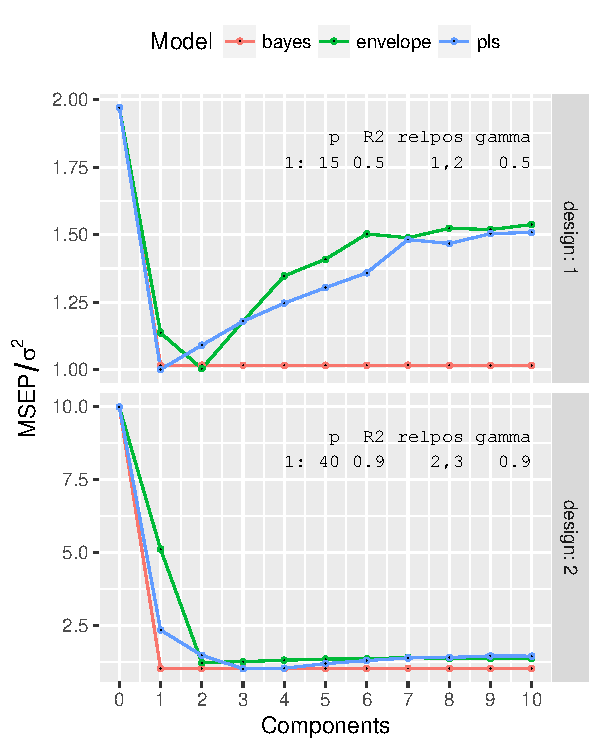
\includegraphics[width=\textwidth]{../pdf/msep-sigma-plot.pdf}
%     \caption{MSEP based on 5,000 test samples}
%     \label{fig:msep}
%   \end{subfigure}
%   \begin{subfigure}[b]{0.5\textwidth}
%     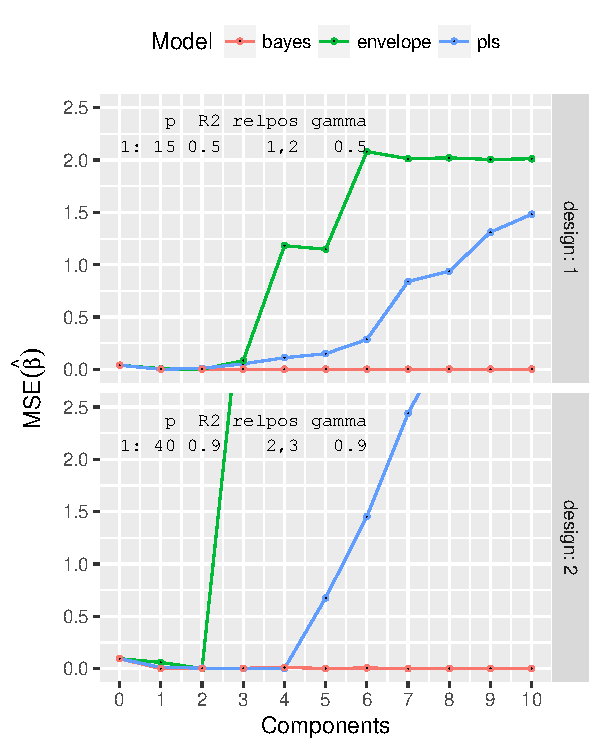
\includegraphics[width=\textwidth]{../pdf/est-error-plot.pdf}
%     \caption{MSE of estimated coefficients ($\hat{\beta}$)}
%     \label{fig:mse_beta}
%   \end{subfigure}
%   \caption{Comparison of Bayes, envelope(MLE) and PLS estimates on the basis of
%     prediction error and estimation error}
% \end{figure}

u Typically, MSEP is lower than that for PLS. A particularly desirable feature of Bayes-PLS is that the MSEP-curve seems to be almost flat for small values of. Thus the error made by choosing a wrong number of components $m$ by crossvalidation must be expected to be small if $m$ is relatively small.

The less desirable featurs of Bayes-PLS is that it requires very heavy computation taking long time with currently available software. The computational burden is largest when $p$ is large. The computation time can be made somewhat  less if we concentrate on the one-component model $m=1$.

\section{Data Simulations for model comparison}

An empirical comparison of these models is conducted based on their ability to
predict test samples. Since, these estimation methods are based on latent
structure, data with diverse properties of latent structure is necessary. For
the simulation of such data, an r-package {\tt simrel} is used. {\tt simrel} is
a simulation tool that can simulate linear model data based on the properties of
latent structure. Apart from the tool, a parameter setup is designed from the
combination of following parameters.

\bigskip

\begin{tabular}{rll}
  Number of training samples       & {\tt n}     & 50 \\
  Number of predictor variables    & {\tt p}     & 15 and 40 \\
  Coefficient of variation         & {\tt R2}    & 0.5 and 0.9 \\
  Position of relevant components  & {\tt relpos}
                                   & $\triangleright$ 1, 2 \;           
                                    $\triangleright$ 1,  3 \; \newline  
                                    $\triangleright$ 2,  3 and \;       
                                    $\triangleright$ 1,  2, 3 \\        
  Decay factor of eigenvalues of X & {\tt gamma} & 0.5 and 0.9
\end{tabular}

\bigskip
 

% \begin{figure}[H]
%   \centering
%   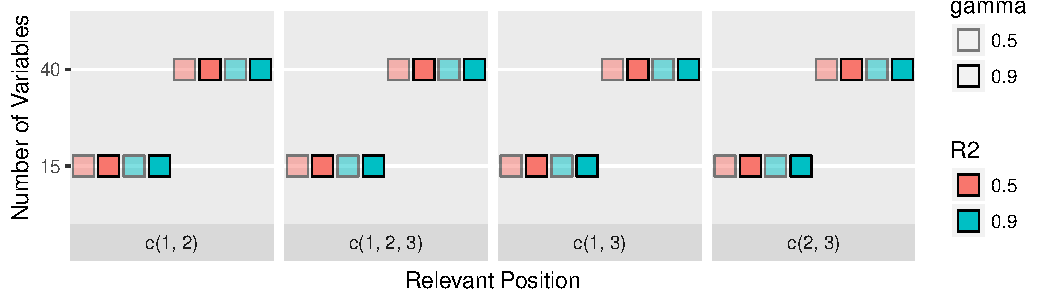
\includegraphics[width=\textwidth]{../pdf/design-plot}
%   \caption{Simulation Design}
%   \label{fig:design}
% \end{figure}

\section{Systematic comparisons}

Solve/Raju: Det er flere estimatorer som det kan v\ae re interessant \aa\ sammenligne her. F\o rst gj\o r MSEP-plott for utvalgte parametersettinger med vanlig PLS, Bayes PLS, muligens SPLS av Chun \& Keles (2010)  (Se R-pakken p\aa\ cran.r-project.org/web/packages/spls.) og maximum likelihood estimatoren (hvis det er mulig \aa\ trekke den ut fra MATLAB-pakken i Cook et al (2014)). Ta med alle metodene i samme plot. 

Kanskje legge til en sammenligning med kryssvaidering for hver enkelt metode. Gj\o r variansanalyse, og ta med middelverdier ved signifikante effekter.

Selvsagt utstrakt bruk av simrel. Kanskje et fraksjonelt design. Vi kan diskutere valg av parametre her, men i utgangspunktet b\o r vi dekke et ganske vidt omr\aa de med $q=p$. Ta med noen virkelig store $p$-verdier (??)  

Virkelig stor $p$ er problematisk av flere grunner, kfr. resultatet til Chun \&
Keles (2010) om inkonsistens av vanlig PLS regresjon når $p/n\rightarrow k>0$ og
det er feil i $x$-variablene. 
\section{Discussion}

There is a vast literature on applications of PLS, not only in chemistry, but in
a large number of applied fields; see for instance Boulesteix \& Strimmer
(2006). Many further references are given in \citet{mehmood2016diversity}
Mehmoood and Ahmed (2015).

Sometimes the issue is prediction, but very often one also see interpretations of scoring plots, loading plots and correlation plots; see for instance Martens \& Martens (2001). Such plots are not unfamiliar to statisticians in principal component connections, but they are much more used by the chemometric society and many scientists find them informative. They are plots of the sample variants of the latent variables and parameters defined by (\ref{wt}), (\ref{pq}) and (\ref{latent}), and thus involve consistent estimates of these quantities when $n\rightarrow\infty$ and probably also in the more general case $p/n\rightarrow 0$.

By comparison there are relatively few papers by mathematical statisticians investigating statistical properties of the partial least squares regression method itself. There are however several investigations on the shrinkage properties of PLS; see Kr\"{a}mer (2007) and references there, and also Foschi (2015) with references. Garthwaite (1994) offered a simple interpretation of PLS. Stone \& Brooks (1990) and Naik \& Tsai (2000)  discuss different generalizations of PLS; in the latter paper also consistency of PLS is proved. Stoica \& Soderstorom (1998) derives asymptotic formulae related to PLS. Chun \& Keles (2010) extends consistency to the case $p/n\rightarrow 0$, introduces a sparse PLS algorithm, and compares methods by simulation.  Kr\"{a}mer \& Sugiama (2011) discusses the degrees of freedom of PLS regression, and uses this concept in model selection. See also references in this last paper.

The purpose of the present article has been to discuss the approach to PLR-regression via model reduction in the random $\bm{x}$ multiple regression model, and to compare estimators in this reduced model....(The rest depends on the results of the simulations.)

\bibliography{references}

\bigskip

\ \\
Inge S. Helland \\
Department of Mathematics \\
\href{http://uio.no}{University of Oslo} \\
POBox 1053 \\
NO-0316 Oslo \\
Norway

\ \\
E-mail: \href{mailto:ingeh@math.uio.no}{ingeh@math.uio.no}


\end{document}
